%%%%%%%%%%%%%%%%%%%% chapter.tex (Chapter 5) %%%%%%%%%%%%%%%%%%%%%%%%%%%%%
% Chapter 5: Deadlock Theory, Turn Models & Adaptive Routing
%%%%%%%%%%%%%%%%%%%%%%%%%%%%%%%%%%%%%%%%%%%%%%%%%%%%%%%%%%%%%%%%%%%%%%%%%

\chapter{Deadlock Theory, Turn Models \& Adaptive Routing}
\label{ch:deadlock_routing}

\author{NoC-Lab Research Consortium}
\institute{NoC-Lab Research Consortium \at Shanghai Jiao Tong University \& International Collaborators, \email{research@network-on-chip.org}}

\maketitle

\abstract*{In packet-switched Networks-on-Chip (NoCs), deadlock represents an unrecoverable failure state in which a set of packets are mutually blocked indefinitely, freezing communication across the silicon die. While Store-and-Forward networks localize buffer dependencies to adjacent nodes, Wormhole Switching dramatically inflates the resource dependency space because packets span multiple physical links simultaneously. This chapter provides a rigorous theoretical and microarchitectural treatment of routing deadlock freedom. We analyze the Dally-Seitz Channel Dependency Graph (CDG) theorem, establish the necessary and sufficient conditions for cycle-free routing, and examine the Glass-Ni Turn Models that deliver partially adaptive routing without virtual channels. We formulate Duato's theorem proving that adaptive subnetworks may contain cycles if an acyclic escape subnetwork is present, and examine the Odd-Even turn model. Finally, we explore state-of-the-art IEEE TCAD and TCAS-II 2026 breakthroughs, addressing protocol-level deadlock in cache-coherent manycores via the PCMT framework and 3D multi-chiplet deadlock avoidance via ScaDA-Rou.}

\abstract{In packet-switched Networks-on-Chip (NoCs), deadlock represents an unrecoverable failure state in which a set of packets are mutually blocked indefinitely, freezing communication across the silicon die. While Store-and-Forward networks localize buffer dependencies to adjacent nodes, Wormhole Switching dramatically inflates the resource dependency space because packets span multiple physical links simultaneously. This chapter provides a rigorous theoretical and microarchitectural treatment of routing deadlock freedom. We analyze the Dally-Seitz Channel Dependency Graph (CDG) theorem, establish the necessary and sufficient conditions for cycle-free routing, and examine the Glass-Ni Turn Models that deliver partially adaptive routing without virtual channels. We formulate Duato's theorem proving that adaptive subnetworks may contain cycles if an acyclic escape subnetwork is present, and examine the Odd-Even turn model. Finally, we explore state-of-the-art IEEE TCAD and TCAS-II 2026 breakthroughs, addressing protocol-level deadlock in cache-coherent manycores via the PCMT framework and 3D multi-chiplet deadlock avoidance via ScaDA-Rou.}

\section{The Deadlock Problem in Wormhole-Switched Fabrics}
\label{sec:ch5_problem}
\index{Deadlock}
\index{Wormhole Switching Dependencies}

In a packet-switched interconnection network, \textbf{deadlock} occurs when a set of concurrent packets cannot make forward progress because each packet holds one or more buffer resources while awaiting buffers held by other packets in the set.

In \textbf{Wormhole Switching}, buffer allocation operates at the flit granularity while routing and channel acquisition occur at the packet level. Consequently, a single packet of length $L$ flits spans across multiple physical links and intermediate routers simultaneously:
\begin{itemize}
    \item The \textbf{Head flit} arbitrates for downstream virtual channels and crossbar ports.
    \item The \textbf{Body flits} trail behind in intermediate router FIFO buffers.
    \item The \textbf{Tail flit} releases channel reservations upon traversing the link.
\end{itemize}
When a Head flit encounters buffer backpressure at a downstream router, the body flits stall in place, holding buffers across the upstream routers. This simultaneous \emph{holding} and \emph{requesting} of distributed resources creates cyclical resource dependency loops.

Architects distinguish deadlock from two related communication anomalies:
\begin{enumerate}
    \item \textbf{Deadlock}: Permanent cessation of forward progress caused by circular resource dependencies.
    \item \textbf{Livelock}: Packets remain in continuous motion across the network but never arrive at their destinations due to unconstrained non-minimal deflection.
    \item \textbf{Starvation}: A packet is permanently denied switch arbitration access due to unfair allocation policies, despite the network remaining active.
\end{enumerate}

\section{The Dally-Seitz Channel Dependency Graph Theorem}
\label{sec:ch5_dally_seitz}
\index{Dally-Seitz Theorem}
\index{Channel Dependency Graph (CDG)}

The foundational mathematical framework for proving deadlock freedom in packet networks was developed by William J. Dally and Charles L. Seitz~\cite{Dally1987}.

\subsection{Formal Definition of the CDG}
Let $I = (V, C)$ be an interconnection network, where $V$ is the set of router nodes and $C$ is the set of directed physical and virtual channels. Let $R: C \times V \to \mathcal{P}(C)$ be the routing function determining permissible egress channels from an ingress channel $c_i \in C$ toward destination $v \in V$.

The \textbf{Channel Dependency Graph (CDG)} $D = (C, E_{CDG})$ is a directed graph where:
\begin{itemize}
    \item Vertices correspond to channels $c \in C$.
    \item A directed edge $(c_i, c_j) \in E_{CDG}$ exists if and only if a packet can transition directly from channel $c_i$ to channel $c_j$ under routing function $R$:
    \begin{equation}
    (c_i, c_j) \in E_{CDG} \iff \exists v \in V \quad \text{such that} \quad c_j \in R(c_i, v)
    \label{eq:ch5_cdg_def}
    \end{equation}
\end{itemize}

\subsection{The Theorem}
\begin{theorem}[Dally \& Seitz, 1987]
A deterministic routing function $R$ for an interconnection network $I$ is deadlock-free if and only if its Channel Dependency Graph $D = (C, E_{CDG})$ has no directed cycles.
\end{theorem}

\begin{proof}
\textbf{Sufficiency ($\Leftarrow$)}: If $D$ has no directed cycles, it is a finite Directed Acyclic Graph (DAG). There exists at least one channel $c_{sink} \in C$ with zero out-degree (delivering to local core memory). A packet occupying $c_{sink}$ cannot be blocked by any other packet in the fabric and will clear in finite time. By topological sorting of the DAG, every channel can be assigned an integer rank $\text{rank}(c_i)$ such that $(c_i, c_j) \in E_{CDG} \implies \text{rank}(c_i) < \text{rank}(c_j)$. Flits on channels of rank $K$ are guaranteed forward progress once channels of rank $> K$ clear. Hence, deadlock is impossible.

\textbf{Necessity ($\Rightarrow$)}: If $D$ contains a directed cycle $c_0 \to c_1 \to \dots \to c_{M-1} \to c_0$, one can construct a traffic state with $M$ packets $P_0, \dots, P_{M-1}$ such that $P_i$ holds channel $c_i$ and requests channel $c_{(i+1) \bmod M}$. If all channels have finite buffer capacity and are full, no packet can advance, producing an unrecoverable deadlock.
\end{proof}

\subsection{Application: Dimension-Order Routing (XY Routing)}
In a 2D Mesh, deterministic XY routing requires packets to exhaust all displacement in the $X$-dimension before turning onto the $Y$-dimension.
\begin{itemize}
    \item \textbf{Allowed Turns}: $(X \to X), (X \to Y), (Y \to Y)$.
    \item \textbf{Prohibited Turns}: $(Y \to X)$ (no turns from $Y$-channels onto $X$-channels).
\end{itemize}
Because $X$-channels never depend on $Y$-channels, all edges in the CDG flow strictly from $X$ to $Y$. The CDG is strictly acyclic, proving that **XY routing is provably deadlock-free on any 2D mesh without requiring virtual channels**.

\section{Glass \& Ni Turn Models for Adaptive Routing}
\label{sec:ch5_turn_models}
\index{Turn Model}
\index{West-First Routing}
\index{North-Last Routing}

While XY routing is deadlock-free, it is strictly non-adaptive: packets cannot route around congested or faulty routers. Christopher J. Glass and Lionel M. Ni~\cite{Glass1994} introduced the **Turn Model**, enabling partially adaptive deadlock-free routing without adding virtual channels.

\subsection{Turn Analysis in a 2D Mesh}
In a 2D Mesh, flits travel in 4 directions: East, West, North, South. There are exactly $4 \times 2 = 8$ possible 90-degree turns:
$$\{E \to N, \quad E \to S, \quad W \to N, \quad W \to S, \quad N \to E, \quad N \to W, \quad S \to E, \quad S \to W\}$$

These 8 turns form two simple directed cycles:
\begin{enumerate}
    \item \textbf{Clockwise Cycle}: $E \to S \to W \to N \to E$ (uses $E \to S, S \to W, W \to N, N \to E$).
    \item \textbf{Counter-Clockwise Cycle}: $E \to N \to W \to S \to E$ (uses $E \to N, N \to W, W \to S, S \to E$).
\end{enumerate}

\begin{theorem}[Glass \& Ni, 1994]
To prevent deadlock in a mesh network, it is necessary and sufficient to prohibit at least one turn from every simple cycle. To maximize routing adaptiveness, exactly one turn from each directed cycle should be prohibited.
\end{theorem}

By prohibiting exactly **2 out of the 8 turns** (one clockwise, one counter-clockwise), the network achieves **75\% (6/8) turn freedom** while completely breaking all dependency cycles!

\subsection{The Canonical 2D Turn Models}
\begin{enumerate}
    \item \textbf{West-First}:
    \begin{itemize}
        \item Prohibited turns: $N \to W$ and $S \to W$.
        \item Rule: If a packet must travel West ($\Delta X < 0$), it must execute all Westward hops first.
        \item Adaptiveness: East-bound packets ($\Delta X > 0$) enjoy 100\% full adaptiveness.
    \end{itemize}
    \item \textbf{North-Last}:
    \begin{itemize}
        \item Prohibited turns: $N \to E$ and $N \to W$.
        \item Rule: Northward hops must be postponed until all East, West, and South hops are complete.
    \end{itemize}
    \item \textbf{Negative-First}:
    \begin{itemize}
        \item Prohibited turns: Transitions from positive directions ($+X, +Y$: East, North) to negative directions ($-X, -Y$: West, South).
        \item Rule: Flits must complete all negative dimension hops before acquiring positive channels.
    \end{itemize}
\end{enumerate}

\section{The Odd-Even Turn Model}
\label{sec:ch5_odd_even}
\index{Odd-Even Routing}

To eliminate the directional asymmetry of the Glass-Ni turn models, Ge-Ming Chiu~\cite{Chiu2000} introduced the \textbf{Odd-Even Turn Model}, where turn restrictions depend on the column coordinate parity ($x \bmod 2$):
\begin{itemize}
    \item \textbf{At Even Columns ($x \bmod 2 == 0$)}: Prohibit $N \to W, S \to W$ and $E \to N, E \to S$.
    \item \textbf{At Odd Columns ($x \bmod 2 == 1$)}: Prohibit $N \to E, S \to E$ and $W \to N, W \to S$.
\end{itemize}
By alternating restrictions between adjacent columns, Odd-Even routing distributes adaptiveness uniformly across East-bound and West-bound flows without requiring virtual channels.

\section{Duato's Theorem for Fully Adaptive Routing}
\label{sec:ch5_duato}
\index{Duato's Theorem}
\index{Escape Virtual Channels}

In 1993, Jos{\'e} Duato~\cite{Duato1993} established a breakthrough result proving that **an adaptive routing function does NOT require an acyclic Channel Dependency Graph to guarantee deadlock freedom**.

\begin{theorem}[Duato, 1993]
An adaptive routing function $R$ for an interconnection network $I$ is deadlock-free if the channel set $C$ can be partitioned into an adaptive channel subset $C_A$ and an escape channel subset $C_E$ ($C = C_A \cup C_E$) such that:
\begin{enumerate}
    \item The escape subnetwork $C_E$ is strictly acyclic under escape routing function $R_E$.
    \item Flits occupying any adaptive channel in $C_A$ are always permitted to transition into $C_E$.
    \item The escape subnetwork provides a connected path between every source and destination pair.
\end{enumerate}
\end{theorem}

Under Duato's paradigm, routers deploy at least 2 Virtual Channels per physical link:
\begin{itemize}
    \item $VC_1 \dots VC_{V-1}$: **Adaptive Subnetwork ($C_A$)**, where packets can take any minimal uncongested channel (cycles permitted in CDG).
    \item $VC_0$: **Escape Subnetwork ($C_E$)**, restricted to strict Dimension-Order (XY) routing (strictly acyclic CDG).
\end{itemize}
If contention builds in $C_A$, flits escape into $VC_0$, where the acyclic escape paths guarantee drain to the destination.

\section{Protocol-Level Deadlock and the PCMT Architecture}
\label{sec:ch5_pcmt}
\index{Protocol Deadlock}
\index{Virtual Networks}
\index{PCMT}

In shared-memory multi-core processors, routing-level deadlock freedom is insufficient to guarantee system forward progress. Cache coherence protocols introduce high-level message dependencies that can cause **Protocol-Level Deadlock**.

\begin{figure}[htbp]
\centering
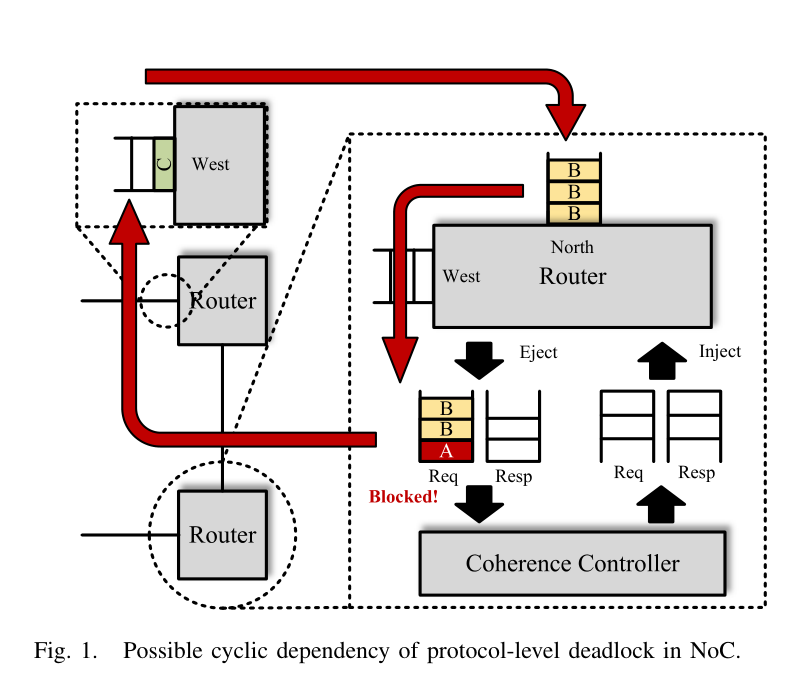
\includegraphics[width=0.48\textwidth]{chapters/ch05-routing-deadlock-theory/figures/pcmt_fig01_protocol_deadlock.png}
\hfill
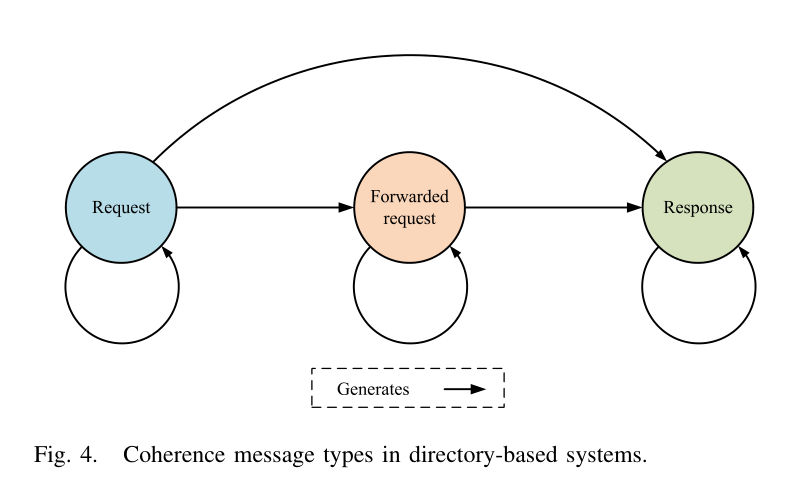
\includegraphics[width=0.48\textwidth]{chapters/ch05-routing-deadlock-theory/figures/pcmt_fig04_coherence_messages.png}
\caption{Protocol-level deadlock in cache-coherent multi-cores: (left) circular dependency loop between coherence Request and Response message buffers; (right) hierarchical message classification in directory-based systems. [Reproduced from: Y. Jia, Z. Zhang, C. Fu, L. Wan, and J. Han, ``PCMT: Prioritizing Coherence Message Types for NoC Protocol-Level Deadlock Freedom,'' \emph{IEEE Trans. Comput.-Aided Design Integr. Circuits Syst.}, Vol.~45, No.~4, pp.~1949--1962, April 2026, DOI: 10.1109/TCAD.2025.3524944. \copyright~2026 IEEE]}
\label{fig:ch5_pcmt_deadlock}
\end{figure}

In directory-based protocols, requests generate forwarded invalidations, which generate responses. If all message types share a common buffer pool, a Request packet cannot be accepted by a core whose output queue is blocked by an outgoing Response packet that cannot enter the congested network.

The traditional mitigation—**Virtual Networks (VNs)**—rigidly isolates Requests, Invalidation, and Responses into dedicated physical VCs. However, Jia et al.~\cite{Jia2026} proved that VNs suffer from severe Head-of-Line blocking and underutilization:

\begin{figure}[htbp]
\centering
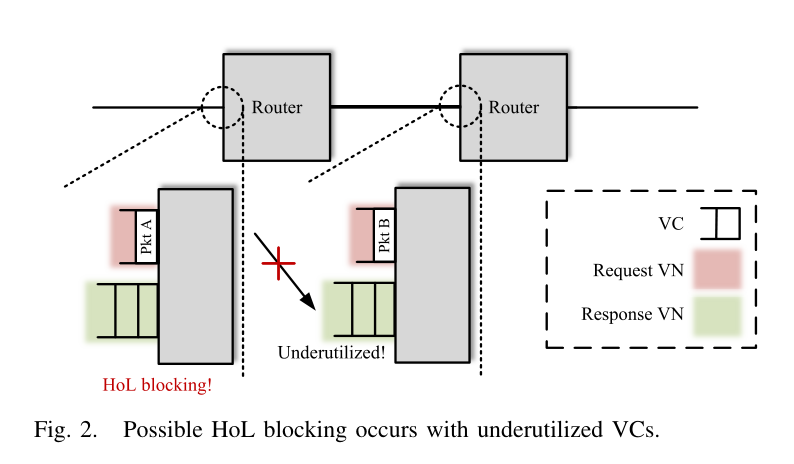
\includegraphics[width=0.55\textwidth]{chapters/ch05-routing-deadlock-theory/figures/pcmt_fig02_hol_blocking.png}
\caption{Underutilization and Head-of-Line blocking in virtual networks. Dedicated partition walls force flits to stall while response VCs remain empty. [Reproduced from: Y. Jia et al., ``PCMT,'' \emph{IEEE Trans. Comput.-Aided Design Integr. Circuits Syst.}, Vol.~45, No.~4, April 2026, DOI: 10.1109/TCAD.2025.3524944. \copyright~2026 IEEE]}
\label{fig:ch5_pcmt_hol}
\end{figure}

Jia et al. introduced **PCMT (Prioritizing Coherence Message Types)**, which eliminates rigid VN partitions in favor of a shared unified buffer pool. By prioritizing Response flits during switch allocation, PCMT drains downstream dependence chains and resolves protocol-level deadlocks while **slashing router input buffer area by up to 63\%**.

\section{3D Multi-Chiplet Deadlock Freedom: ScaDA-Rou}
\label{sec:ch5_scada}
\index{3D Multi-Chiplet Routing}
\index{ScaDA-Rou}

In 3D multi-chiplet systems, vertical Through-Silicon Vias (TSVs) introduce cross-plane dependencies that interact catastrophically with planar turn models.

\begin{figure}[htbp]
\centering
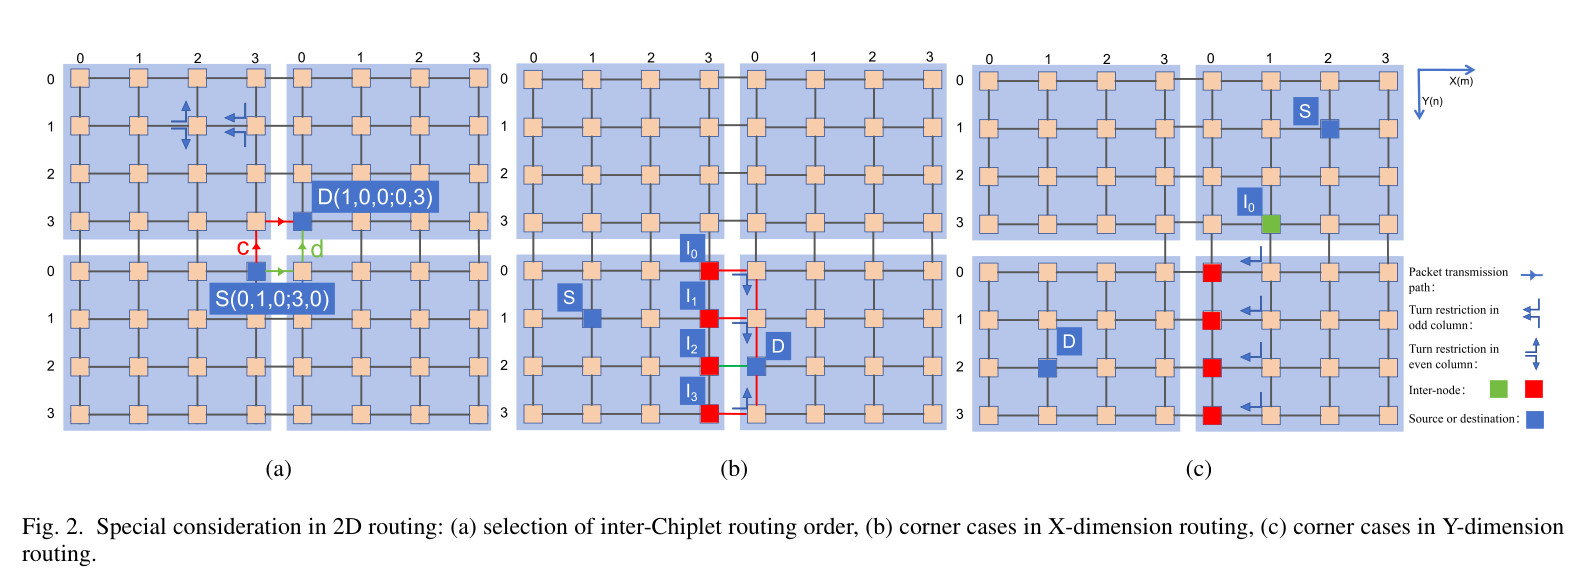
\includegraphics[width=0.85\textwidth]{chapters/ch05-routing-deadlock-theory/figures/scada_fig02_turn_model_rules.png}
\caption{ScaDA-Rou routing rules for 3D multi-chiplet systems: (a) inter-chiplet routing order; (b) boundary corner cases in $X$-dimension; (c) boundary corner cases in $Y$-dimension. [Reproduced from: L. Zhu, H. Gu, Y. Tan, and G. Zhang, ``ScaDA-Rou: A Scalable, Deadlock-Free, and Adaptive Routing for 3-D Multi-Chiplet System,'' \emph{IEEE Trans. Circuits Syst. II, Express Briefs}, Vol.~73, No.~4, pp.~433--437, April 2026, DOI: 10.1109/TCSII.2025.3526101. \copyright~2026 IEEE]}
\label{fig:ch5_scada}
\end{figure}

Zhu et al.~\cite{Zhu2026} proposed **ScaDA-Rou**, combining in-plane turn model restrictions with cross-plane virtual network partitioning. By separating the virtual channels used for the source and destination planes of vertical packets, ScaDA-Rou eliminates 3D cyclic dependencies and achieves an **89.2\% latency improvement** over baseline architectures.

\section{Routing Algorithm Comparative Matrix}
\label{sec:ch5_matrix}

Table~\ref{tab:ch5_routing} summarizes the properties of the foundational and modern routing algorithms.

\begin{table}[htbp]
\centering
\caption{Comparative Matrix of On-Chip Routing Algorithms}
\label{tab:ch5_routing}
\begin{tabular}{lcccc}
\toprule
\textbf{Routing Scheme} & \textbf{Turn Prohibitions} & \textbf{Min. VCs} & \textbf{Adaptiveness} & \textbf{Throughput Gain} \\
\midrule
Dimension-Order (XY) & $Y \to X$ prohibited & 1 & Deterministic & Baseline \\
West-First (Glass-Ni) & $N \to W, S \to W$ & 1 & Partially Adaptive & +25\% \\
North-Last (Glass-Ni) & $N \to E, N \to W$ & 1 & Partially Adaptive & +25\% \\
Negative-First & $+ \to -$ prohibited & 1 & Partially Adaptive & +20\% \\
Odd-Even (Chiu) & Column-parity dependent & 1 & Partially Adaptive & +35\% \\
Duato FAR + XY Escape & None in $C_A$ & 2 & Fully Adaptive & +75\%--100\% \\
PCMT (Jia et al., 2026) & Priority-preemptive & Unified Pool & Protocol Deadlock-Free & -63\% Area \\
\bottomrule
\end{tabular}
\end{table}

\section{Exercises and Review Questions}
\label{sec:ch5_exercises}

\begin{enumerate}
    \item \textbf{CDG Construction}: For a $2 \times 2$ 2D Mesh, enumerate all directed physical channels and draw the Channel Dependency Graph under fully adaptive minimal routing. Identify the cycle and show how West-First routing breaks it.
    \item \textbf{Duato Theorem Dynamics}: In a network deploying Duato's escape routing, why must packets on the escape subnetwork ($VC_0$) be prohibited from transitioning back into the adaptive subnetwork ($VC_1$)?
    \item \textbf{Protocol Deadlock Scenario}: Sketch a sequence of coherence transactions in a MESI protocol where all routers utilize deadlock-free XY routing, yet the system suffers protocol-level deadlock due to full request buffers.
\end{enumerate}
